\chapter{Design specification}\label{ch:design}

\section{Overview}

This section describes the design work done through the project as well as the tools used to carry that labor and the results of it. The chapter covers the following topics:

\begin{itemize}
\item \textbf{Architecture of the system:} The chosen architecture of the system is described, together with the reasons and advantages of the design.
\item \textbf{Design of the ontology:} The final design of the ontology is described, as well as it's advantages in front of other data modeling paradigms.
\item \textbf{Design of the central server:} The class design of the server is detailed in this section.
\item \textbf{Design of the web application:} The class design of the web application is detailed in this section, as well as the interface design.
\item \textbf{Design of the mobile application:} The class design of the mobile application is detailed in this section, as well as the interface design.
\item \textbf{Development environment:} The list of technologies employed in the project is detailed, briefly explaining the role of each tool.

\end{itemize}

\section{System architecture}\label{sec:designarch}

Figure \ref{fig:architecture} shows the architecture chosen for the system. This architecture comprises the following elements:

\begin{itemize}
\item A central server
  \begin{itemize}
  \item Web server
  \item SPARQL endpoint
  \item REST API
  \item Data agregator
  \item Database connector
  \end{itemize}
\item A semantic spatial storage system which contains the ontology
\item A web client used as the main interface of the system
\item A mobile application to support the browser based one
\end{itemize}

\begin{figure}[ht]
  \centering
  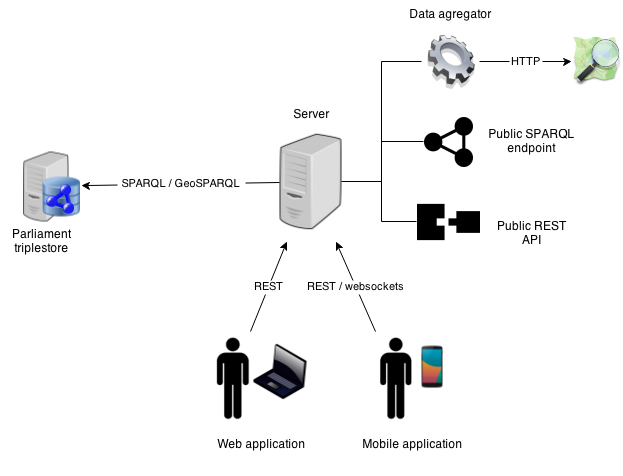
\includegraphics[width=.8\textwidth]{fig/architecture}
  \caption{Architecture design of the system}
  \captionsetup{font={footnotesize,bf,it}}
  \label{fig:architecture}
\end{figure} 

\subsection{Central server}

The central server is the core component of the system. It implements most of the functionality on the system and provides data to the client. It also analyzes the trails uploaded to the system and takes care of the communication with the database. The server is divided into several logical software pieces, which are described below.

\subsubsection*{Database connector}

The database connector implements the functionality needed to connect with the semantic data store. In essence, this means that it takes the requests from the users and transforms them into SPARQL queries. Then it takes the results provided by the database and converts them into a format that the server can process.

\subsubsection*{The data agregator}

This component has the function of querying external data sources and adapting the results to the data model of the system. It is independent of the rest of components of the server, since instead of being available to receive requests it will just run on demand. The component makes HTTP queries to the different APIs and endpoints on the web, for example OpenStreetMap and Geonames, and aggregates the data to the database.

\subsubsection*{REST API}

The API provides the basic means of accessing the information on the system. It is used by both clients to communicate with the server. It can be used for read, write and update operations, however, delete operations are not contemplated.

\subsubsection*{The SPARQL endpoint}

This endpoint just routes SPARQL queries done to it to the database. Its role is related to filtering the queries that seek to write and to ensure that no petition is going to break the integrity of the data in the database.

\subsection{Semantic spatial storage system}

This component of the system is mostly third party software. It consists on a triple store, a data storage system that stores RDF data; a reasoner supporting OWL and GeoSPARQL and an HTTP SPARQL endpoint. This component also englobes the ontology designed to define the data model of the system. This ontology is described in detail in section \ref{sec:ontdesign}.

\subsection{Web client}

The web client is the main interface though which the system is accessed. It communicates with the server through a REST API and offers most of the functionality of the system to the users.

The client may be used from desktop browsers or mobile browser with no restrictions. More details on the design of the client can be found on section \ref{sec:webappdesign}.

\subsection{Mobile application}

The mobile client provides the functionality that the web application cannot. It provides real time functions by using a websocket API that the server exposes. The design of this component is detailed in section \ref{sec:mobileappdesign}.

\section{Design of the ontology}\label{sec:ontdesign}

The ontology designed in the project represents specific knowledge related to the domain of Trails, Points of Interest and GPS data in general. It uses external ontologies as a base, in order to ease the sharing of information and the publishing of the dataset at Linked Open Data.

\begin{figure}[ht]
  \centering
  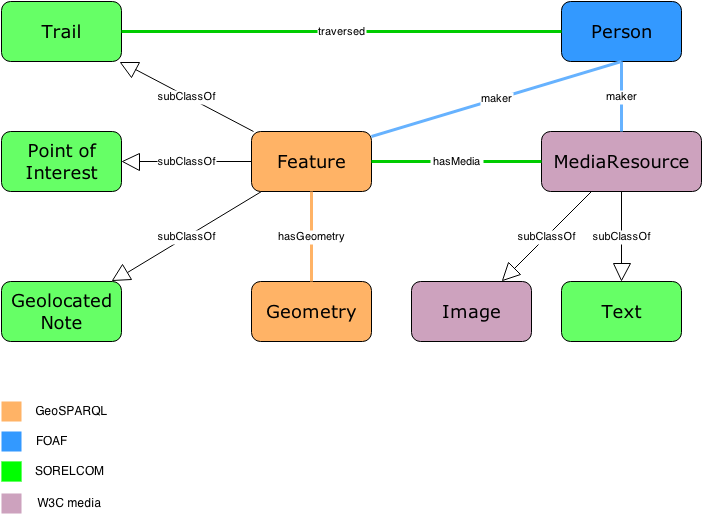
\includegraphics[width=.8\textwidth]{fig/sorelcom-ontology}
  \caption{The SORELCOM ontology}
  \captionsetup{font={footnotesize,bf,it}}
  \label{fig:sorelcom-ontology}
\end{figure} 

Figure \ref{fig:sorelcom-ontology} provides a graphical representation of classes on the SORELCOM ontology. As shown on the figure, classes from three vocabularies are reused. The FOAF vocabulary is used to obtain a representation of the users of the platform, the GeoSPARQL vocabulary is used as a base for all the resources with a spatial character and the W3C media vocabulary is used to represent the media resources on the platform.

The focus of the design is to reuse as many well known vocabularies as possible and defining the needed classes, relations and properties to satisfy the requirements of the ontology 4 to 10, defined in chapter \ref{ch:requirements}.

\subsection{Class hierarchy}

The ontology defines a series of classes for the representation of specific spatial features present in the domain of the application. The classes are listed below:

\begin{description}
\item[\texttt{sorelcom:Trail}] A trail represents a path in the world. In the context of the application, a trail can be interpreted as a path that a user has traversed or as a simple route that is indicated by a user, however, the ontology does not specify that a trail should have any of these meanings.

\item[\texttt{sorelcom:PointOfInterest}] A Point of Interest is a feature in the world that may result of some interest for a person. There is no specification on what can be the interest a person may have on the feature, thus a point of interest may be anything from a monument to a restaurant.

\item[\texttt{sorelcom:GeolocatedNote}] A Geolocated Note is a message with a spatial context. This message is left by a person at a specific location, and can be viewed by any person or just a specific group depending on its privacy settings. The message on a note may be formed by text, images, video or any combination of them.
\end{description} 

In addition to the core types on the vocabulary, other classes obtained from external ontologies will be used or extended to represent different types of resources on the ontology. The additional classes used are the following:

\begin{description}
\item[\texttt{foaf:Person}] This class is used to classify resources as persons. Any user on the system will be classified as person. The class is defined in the FOAF vocabulary.

\item[\texttt{geo:Feature}] A feature is any object in the real world that has a spatial representation. \textit{Trails}, \textit{Points of Interest} and \textit{Geolocated Notes} are all types of Features. This class is defined in the GeoSPARQL vocabulary.

\item[\texttt{geo:Geometry}] In the GeoSPARQL ontology, a geometry is used to give a spatial representation to a Feature. Without a associated feature, geometries are not resources on the real world.

\item[\texttt{media:MediaResource}] A media resource is a representation of a media object, such as a image or a video. Media resources refer to the images, posts and videos saved in the system.

\item[\texttt{media:Image}] A image is a specialized media resource, which refers to a image. It is used in conjunction with the \texttt{sorelcom:Text} class to represent the specific type of a media in the system.
 
\end{description}

\subsection{Properties}

Most of the work on the design of the ontology consists on the creation of properties which relate the resources to the information that they must contain. Still, many of the properties used in the data model of the platform are obtained from external vocabularies.

The properties defined for the SORELCOM vocabulary are listed below, together with a table representing how the information about those resources is stored in the data model:

\subsubsection*{Feature properties}

\begin{description}
\item[\texttt{sorelcom:name}] Property representing the human readable name of a feature. 
\item[\texttt{sorelcom:description}] Property representing a textual description of a feature.
\item[\texttt{sorelcom:hasMedia}] Property relating a feature to the media associated. It is the inverse of \texttt{sorelcom:mediaOf}.
\end{description}

\subsubsection*{Trail properties}

\begin{description}
\item[\texttt{sorelcom:difficulty}] Property representing the difficulty score of a trail. This score is a integer from 0 to 100, the higher the difficulty the higher the number. A trail may only have one difficulty.
\item[\texttt{sorelcom:maximumAltitude}] Property representing the altitude of the highest point of a trail.
\item[\texttt{sorelcom:minimumAltitude}] Property representing the altitude of the lowest point of a trail.
\item[\texttt{sorelcom:totalDistance}] Property representing the total distance in meters that must be traversed from the starting point of a trail to the end of it.
\item[\texttt{sorelcom:ascendingDistance}] Property representing the sum of the distance in meters of the segments of the trail which are ascendant .
\item[\texttt{sorelcom:descendingDistance}] Property representing the sum of the distance in meters of the segments of the trail which are descendant.
\item[\texttt{sorelcom:circular}] Property representing if the starting point and end point of a trail are the same.
\item[\texttt{traversedBy}] Property relating a trail to the users who have traversed it.
\end{description}

Information about how trails are represented on the system can be found on table \ref{tab:trail}.

\begin{table}[ht]
  \centering
  \caption{Trails on the SORELCOM data model.}\label{tab:trail}
  \begin{tabular}{llll}
    \toprule
      \textbf{Property} & \emph{domain}  & \emph{range} & \emph{information}\\
    \midrule
      sorelcom:name & geo:Feature  & string & name \\
      sorelcom:description & geo:Feature & string  & description \\
      sorelcom:difficulty & sorelcom:Trail & integer & difficulty \\
      sorelcom:maximumAltitude & sorelcom:Trail & float & maximum altitude \\
      sorelcom:minimumAltitude & sorelcom:Trail & float & minimum altitude \\
      sorelcom:ascendingDistance & sorelcom:Trail & integer & ascending distance \\
      sorelcom:descendingDistance & sorelcom:Trail & integer & descending distance \\
      sorelcom:hasMedia & geo:Feature & ma:Media & images, posts \\
      foaf:maker & Thing & foaf:Person & author \\
      sorelcom:traversedBy & sorelcom:Trail & foaf:Person & persons who traversed it \\ 
      geo:hasGeometry & geo:Feature & geo:Geometry & spatial representation \\
    \bottomrule
  \end{tabular}
\end{table}

\subsubsection*{Point of interest properties}

\begin{description}
\item[\texttt{sorelcom:altitude}] Property representing altitude of the point. 
\item[\texttt{sorelcom:category}] Property representing the category of the point of interest.
\end{description}

Information about how points of interest are represented on the system can be found on table \ref{tab:poi}.

\begin{table}[ht]
  \centering
  \caption{Points of interest on the SORELCOM data model.}\label{tab:poi}
  \begin{tabular}{llll}
    \toprule
      \textbf{Property} & \emph{domain}  & \emph{range} & \emph{information}\\
    \midrule
      sorelcom:name & geo:Feature  & string & name \\
      sorelcom:description & geo:Feature & string  & description \\
      sorelcom:altitude & sorelcom:PointOfInterest & float & altitude \\
      sorelcom:category & sorelcom:PointOfInterest & string & category \\
      sorelcom:hasMedia & geo:Feature & ma:Media & images, posts \\
      foaf:maker & Thing & foaf:Person & author \\
      geo:hasGeometry & geo:Feature & geo:Geometry & spatial representation \\
    \bottomrule
  \end{tabular}
\end{table}

\subsubsection*{Geolocated Note properties}

\begin{description}
\item[\texttt{sorelcom:range}] Property representing range of action of a Geolocated Note. 
\item[\texttt{sorelcom:public}] Property representing if the note is public.
\item[\texttt{sorelcom:targets}] Property relating the note to the persons that should receive it. It exists only when the note is not public.
\end{description}

Information about how geolocated notes are represented on the system can be found on table \ref{tab:note}.

\begin{table}[ht]
  \centering
  \caption{Geolocated notes on the SORELCOM data model.}\label{tab:note}
  \begin{tabular}{llll}
    \toprule
      \textbf{Property} & \emph{domain}  & \emph{range} & \emph{information}\\
    \midrule
      dcterms:created & Thing & date & creation time \\
      dcterms:valid & Thing & date or integer & duration \\
      sorelcom:public & sorelcom:GeolocatedNote & boolean & privacy level \\
      sorelcom:radius & sorelcom:GeolocatedNote & integer & action radius \\
      sorelcom:hasMedia & geo:Feature & ma:Media & text, multimedia \\
      foaf:maker & Thing & foaf:Person & author \\
      geo:hasGeometry & geo:Feature & geo:Geometry & spatial representation \\
    \bottomrule
  \end{tabular}
\end{table}

\subsubsection*{Person properties}

\begin{description}
\item[\texttt{sorelcom:hasTraversed}] Property relating a Person to the trails it has traversed.
\item[\texttt{sorelcom:trailBuddyOf}] Property relating a Person to his/her trail buddies, that is, people who are usual sports or tourism mates.
\end{description}

Information about how persons are represented on the system can be found on table \ref{tab:user}.

\begin{table}[ht]
  \centering
  \caption{Persons on the SORELCOM data model.}\label{tab:user}
  \begin{tabular}{llll}
    \toprule
      \textbf{Property} & \emph{domain}  & \emph{range} & \emph{information}\\
    \midrule
      foaf:nick & foaf:Person  & string & nickname \\
      foaf:mbox & foaf:Person  & string & email \\
      foaf:firstName & foaf:Person  & string & first name \\
      foaf:familyName & foaf:Person  & string & family name \\
      foaf:depiction & foaf:Person  & foaf:Image & avatar \\
      sorelcom:trailBuddyOf & foaf:Person  & foaf:Person & trail buddies \\
      sorelcom:hasTraversed & foaf:Person & sorelcom:Trail & traversed trails \\
      foaf:weblog & foaf:Person  & URI & external homepage \\
      foaf:made & foaf:Person  & Thing & features and media \\
    \bottomrule
  \end{tabular}
\end{table}

\subsubsection*{Media properties}

\begin{description}
\item[\texttt{sorelcom:mediaOf}] Property relating a media resource to the feature it belongs to.
\end{description}

Information about how media resources are represented on the system can be found on table \ref{tab:media}. Media resources are divided into images, text and video, however, for convenience purposes all of them are presented in a single table. The only properties that are not shared among all media resource types are the content and the download link. The content is only used in the text, while the download link is used on media images and video.

\begin{table}[ht]
  \centering
  \caption{Media on the SORELCOM data model.}\label{tab:media}
  \begin{tabular}{llll}
    \toprule
      \textbf{Property} & \emph{domain}  & \emph{range} & \emph{information}\\
    \midrule
      foaf:maker & Thing & foaf:Person & author \\
      ma:description & ma:MediaResource & string & content \\
      ma:locator & ma:MediaResource & URI & download link \\
      dcterms:created & Thing & datetime & addition date \\
      sorelcom:mediaOf & ma:MediaResource & geo:Feature & feature \\
    \bottomrule
  \end{tabular}
\end{table}

\subsection*{Inference mechanism}

In order to get the maximum benefit from the semantic dataset the ontology has been defined using OWL. Due to this, several inference mechanism have been available during the design process, however, only a subset of them have been used. The following inference mechanisms have been used:

\begin{description}
\item[Sub classes] All resources which are instanced of a certain class A are also instances of the classes A is subclass of. This property is provided by RDF schema (see section \ref{sec:rdf} for more information). In RDF it is possible to use multiple inheritance, meaning that a class can be subclass of more than one class.
\item[Disjoint classes] A group of disjoint classes indicate that a resource of one class of the group cannot be of another class on the group
\item[Sub properties] Subproperty relations are the analogous of subclass relations when referring to resources of type property. It is also provided by RDF schema.
\item[Function properties] A functional property is a property that can only appear once in the triples of a certain resource. It is provided by OWL lite.
\item[Inverse properties] When a resource A is related to B by a property P1, then B is related to A by the property P2 inverse of P1. It is provided by OWL lite.
\item[Symmetric property] When a resource A is related to B by a symmetric property P, then B is related to A also by P.

\end{description}

Table \ref{tab:inferencecls} shows the inference rules used on the classes of the ontology and \ref{tab:inferenceprop} shows the inference rules used on the properties of the data model.

\begin{table}[ht]
  \centering
  \caption{Inferences used on the SORELCOM ontology classes.}\label{tab:inferencecls}
  \begin{tabular}{llll}
    \toprule
      \textbf{Class} & \emph{inference type}  & \emph{Related class}\\
    \midrule
      sorelcom:Trail & subclass of & geo:Feature \\
      sorelcom:PointOfInterest & subclass of & geo:Feature \\
      sorelcom:GeolocatedNote & subclass of & geo:Feature \\
      sorelcom:Text & subclass of & ma:MediaResource \\
      sorelcom:Trail & disjoint with & sorelcom:PointOfInterest \\
      sorelcom:Trail & disjoint with & sorelcom:GeolocatedNote \\
      sorelcom:GeolocatedNote & disjoint with & sorelcom:PointOfInterest \\
    \bottomrule
  \end{tabular}
\end{table}

\begin{table}[ht]
  \centering
  \caption{Inferences used on the SORELCOM ontology classes.}\label{tab:inferenceprop}
  \begin{tabular}{llll}
    \toprule
      \textbf{Property} & \emph{inference type}  & \emph{Related property}\\
    \midrule
      sorelcom:trailBuddyOf & sub property of & foaf:knows \\
      sorelcom:trailBuddyOf & symmetric property \\
      sorelcom:hasTraversed & inverse property of & sorelcom:traversedBy \\
      sorelcom:hasMedia & inverse property of & sorelcom:mediaOf \\
      sorelcom:difficulty & functional property \\
      sorelcom:maximumAltitude & functional property \\
      sorelcom:minimumAltitude & functional property \\
      sorelcom:totalDistance & functional property \\
    \bottomrule
  \end{tabular}
\end{table}

\subsection{Advantages of ontology based design}

The data model on the platform has been designed based on a ontology, mainly to follow the best practices of Linked Open Data. However, there are other alternatives, for instance, using a relational database and a RDF mapper. Mappers, for example, D2RQ expose the data on a relational database as a virtual RDF graph, allowing to query this data using SPARQL. This mappers exist to allow Semantic Web application to access the information stored on relational systems \cite{d2rq}.

Even with this alternatives, the choice to use a completely semantic system over a relational database was made. This choice came with some disadvantages, the main of them being an increased of the complexity of the system. RDF lacks support on programming platforms compared to relational database systems, thus the amount of coding needed increases. Besides, the current standard for the creation of GIS systems, the PostGIS \cite{postgis} extension for the PostgreSQL \cite{postgres} cannot be used. The rest of the spatial databases, including the semantic ones lack support and tools to work with, which has caused an increase in development times.

However using ontologies to define the data model of the platform brings several benefits. The main benefits are detailed in this section.

\subsubsection*{Inference of new knowledge from the existing one}

The main advantage of the ontology based data model design is the possibility of inferring knowledge, that is, creating new knowledge from the existing data. This process usually implies the creation on new triples from the existing triples on the dataset which can be done in two different manners. The first way consists on running the inference process every time a query is made and aggregating the new triples to the results returned. This saves space on the data store but in exchange it increases computation time, for which it is not a very used technique. The more popular approach is running the inference when data is added to the store and generating new statements which will also be saved. This increases space used and time for processing write operation, however, since read operations are usually way more common than read operations it pays off.

This inference is usually done by specialized reasoning software such as the Pellet OWL 2 reasoner \cite{pelletweb}. The data store to be used, Parliament, provides its own reasoner. Parliament's reasoner supports OWL DL inference done when triples are inserted into the data store. The process exploits inference properties like the ones detailed on the previous section to deduce new knowledge, for example, if a property is specified to have a certain domain, then when a triple with that property is inserted into the dataset it is possible to infer that the subject is of the types on the domain of the property. A graphical example of a simple inference can be found in figure \ref{fig:simple-inference}. This example, shows how using inverse relation properties it is possible to obtain inverse properties needing only to specify one end of the relation.

\begin{figure}[ht]
  \centering
  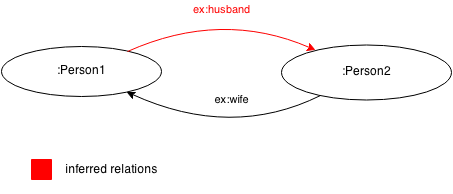
\includegraphics[width=.6\textwidth]{fig/simple-inference}
  \caption{Inference of the husband relation as inverse of the wife relation}
  \captionsetup{font={footnotesize,bf,it}}
  \label{fig:simple-inference}
\end{figure}

Many types of inferences are possible. The inference of the classes of a resource depending on a class hierarchy can be done; the example in figure \ref{fig:inference-hierarchy} shows the usage of the SORELCOM ontology to infer the classes of a resource. Combinations of different inference properties can be used to express complex relations. In figure \ref{fig:complex-inference} inverse and transitive properties together with ranges and domains, are combined to infer knowledge on a small RDF graph.

\begin{figure}[ht]
  \centering
  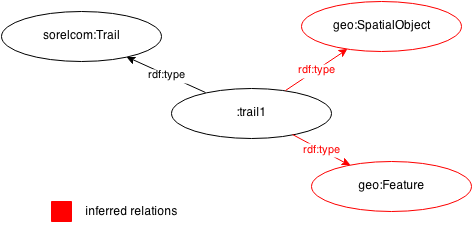
\includegraphics[width=.6\textwidth]{fig/inference-hierarchy}
  \caption{Inference of all the classes of a Trail}
  \captionsetup{font={footnotesize,bf,it}}
  \label{fig:inference-hierarchy}
\end{figure}

\begin{figure}[ht]
  \centering
  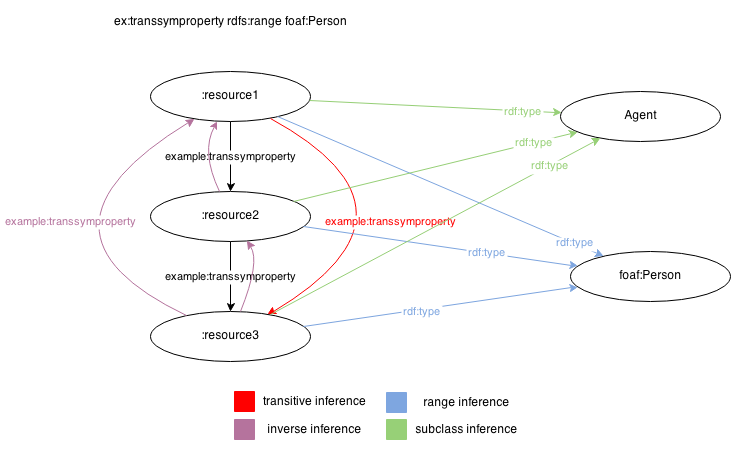
\includegraphics[width=.6\textwidth]{fig/complex-inference}
  \caption{Inference of the husband relation as inverse of the wife relation}
  \captionsetup{font={footnotesize,bf,it}}
  \label{fig:complex-inference}
\end{figure}

Depending on the describing language used, it is possible to create very complex rules, and the inference engine will automatically process all of them. This is one of the biggest advantages over relational database systems where a high amount of relations would need to be defined to encode the complex relations that can be represented in a ontology based system and allows to build complex queries.

\subsubsection{Schema and data separation and reusability}

Ontologies provides mean for reusing other data models, since it is possible to import ontologies into another one. This way, it is possible to use already defined concepts without the need to develop vocabularies for them. One example of this can be found in the SORELCOM vocabulary, where the FOAF, GeoSPARQL, DC and W3C media ontologies are reused.

Besides, this allows separation between the data model and the actual data. In relational database management systems, the structure of the data is physically created on the system itself (for example, a file for each table) and it is not fully supported to import the model of one database to another. When using ontology based databases, the data model is represented by a ontology which can be imported into any data store, thus it is possible to reuse the schema among several different databases.

\subsubsection{Linked Open data}

Ontologies are a tool that facilitate the publishing of Linked Open Data. The inference mechanisms used on these ontologies are not so relevant in this case, however the concepts expressed are crucial. Ontologies allow reusing other vocabularies to express the data model, which is a key point when developing a linked model.

Linked data refers to a set of best practices to publish and interlink structured data for access by both humans and machines via RDF. In order to do this it is necessary to make use of URIs as a real unique identifier, there is no point if a relation that expresses that two persons know each other has a different URI in every dataset. In order to avoid this, well known vocabularies, such as FOAF, and these concepts and relations are uniform among most if not all datasets. This is only possible when using ontology based design, for only ontologies allow this level of reusing.

\section{Design of the central server}\label{sec:serverdesign}

\section{Design of the web application}\label{sec:webappdesign}

\section{Design of the mobile application}\label{sec:mobileappdesign}

\section{Development environment}

The tools and development environment used during the design process have been the following:

\begin{itemize}
\item Prot\'eg\'e-OWL 4.3
\item UML 2
\item Sass 3.8.8
\item Twitter Bootstrap 3.1.1
\end{itemize}

\subsection{Prot\'eg\'e-OWL}

Prot\'eg\'e is an open-source ontology editor and framework for building intelligent systems\cite{protege1}. The traditional architecture of the editor is based on frames \cite{protege2}, however, with the standardization of OWL (see section \ref{sec:owl}) support for this language was added to the framework \cite{protege3}.

The current version of Prot\'eg\'e can be used to edit classes and their characteristics, to access different reasoning engines, to edit and execute queries and rules and to visualize relationships between concepts. The tool has been widely adopted by the Semantic Web ontologists, for all their utilities and because it has been adopted among the W3C recommendations \cite{protege4}.

The tool provides a graphical user interface, which can be seen in figure \ref{fig:protege}. Through this editor, other vocabularies can be imported, in addition to create classes and properties for a new ontology and defining restrictions and relations among them. This tool has been used to create the SORELCOM ontology on the project.

\begin{figure}[ht]
  \centering
  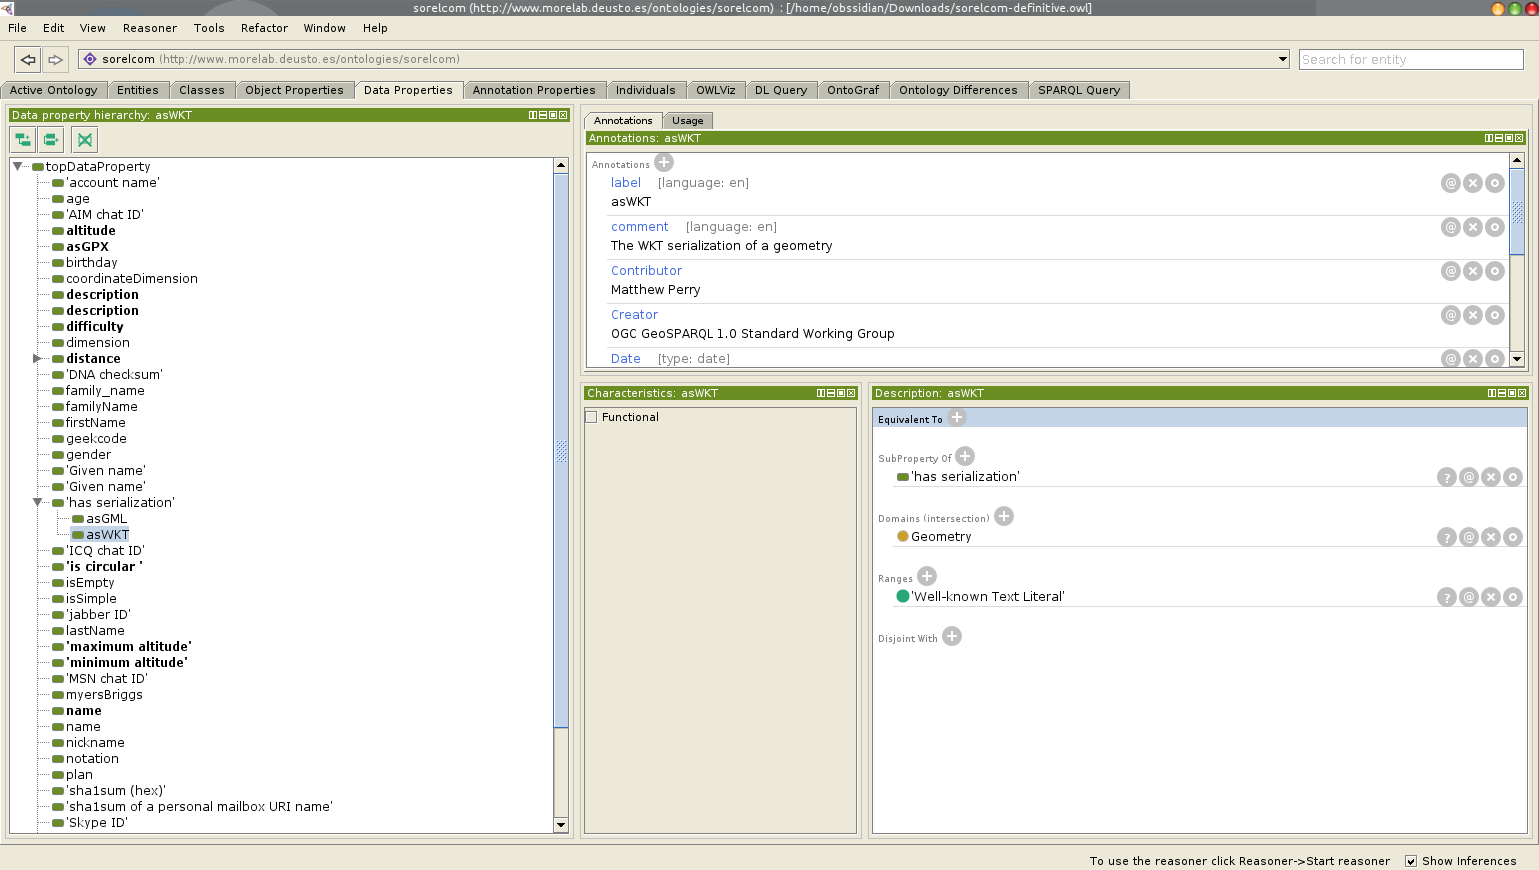
\includegraphics[width=.8\textwidth]{fig/protege}
  \caption{The Prot\'eg\'e OWL ontology editor}
  \captionsetup{font={footnotesize,bf,it}}
  \label{fig:protege}
\end{figure} 

\subsection{UML}

The Unified Modeling Language (UML) is a general-purpose visual modeling language used to specify, visualize, construct and document the artifacts of a software system. It is used to capture decisions and provide understanding of the architecture and class design of the system \cite{uml}. 

UML can be used to capture information about the static design and dynamic behavior of the system and its components through different types of diagram. It is a standard used and accepted worldwide, thanks to which it can be used to expose and interchange information about system designs.

All the component and class diagrams presented in this document have been modeled according to UML standards.

\subsection{SASS}

CSS (Cascading Style Sheet) is a stylesheet language specification used to describe the presentation of documents written in a markup language. It is the technology used to describe the appearance of web pages \cite{css}. SASS \cite{sass} which stands for Syntactically Awesome Style Sheets is a extension and preprocessor for the CSS language which aims to cut on developing times and improve stylesheet maintainability. 

CSS preprocessors have become very popular lately among web developers for various reasons. First, they provide functionality that allows to programatically define styles for a web page instead of just describing, such as variables and functions. Second, these extensions improve code readability and reduce the size of the produced stylesheets. Finally, they follow the principle of DRY (dont repeat yourself), allowing to define the appearance of document without repeating directives. An example of SASS to CSS transformation can be found in figure \ref{fig:sass}.

\begin{figure}[ht]
  \centering
  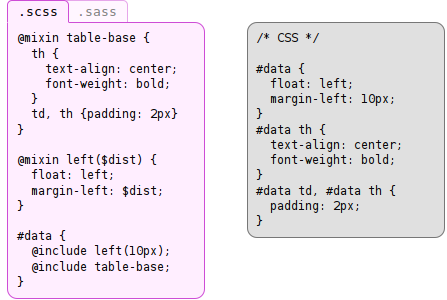
\includegraphics[width=.8\textwidth]{fig/sass}
  \caption{SASS to CSS transformation}
  \captionsetup{font={footnotesize,bf,it}}
  \label{fig:sass}
\end{figure} 

This technology has been used in the project to define the appearance of both the mobile and the web interface.

\subsection{Twitter Bootstrap}

Even with the use of preprocessors, the time it takes to design the appearance of a HTML based application is considerable. In big enough project, specialized designers are employed for the interface design of the application, however on smaller scale projects it has become more usual to use a CSS framework to produce acceptable, if not original, appearances for the user interfaces.

Twitter Boostrap is one of the most, is not the most popular of these frameworks. It provides a set of CSS classes, default styles and JavaScript functions to develop responsive web applications. It has been used in this project to ease the adaptability of the web application interface on all kind of devices.
